\lab{Algorithms}{QR Decomposition using Householder reflectors}{QR Decomposition using Householder reflectors}
\objective{Use orthonormal transformations to perform QR decomposition.}
\label{lab:Canonical Transformations}

\section*{Orthonormal transformations}
Recall that a matrix $Q$ is \emph{unitary} if $Q^\mathsf{H} Q = I$ or for real matrices,
$Q^T Q = I$.
For the real case we say that such a matrix is \emph{orthonormal}.

Unitary transformations have the very desirable property of being numerically stable.
The number $\kappa(A) = \norm{A} \norm{A^{-1}}$ is called the \emph{condition number} of $A$.
We'll discuss condition number more in another lab; for now, all you need to know is that if $\kappa(A)$ is small, then calculations involving $A$ are less susceptible to numerical errors.
For the induced 2-norm, it holds that $\norm{Q}=1$ when $Q$ is unitary.
The Cauchy-Schwarz inequality $\norm{AB} \leq \norm{A} \norm{B}$ also holds for this norm, and
so it follows that $\kappa(A) = \norm{A} \norm{A^{-1}} \geq \norm{A A^{-1}} = \norm{I} = 1$.
Note that if $Q$ is unitary, $Q^{-1} = Q^\mathsf{H}$ and $Q^\mathsf{H}$ is also unitary, so $\kappa(Q) = \norm{Q} \norm{Q^\mathsf{H}} = 1$.
This means that orthonormal matrices have the smallest possible condition number.

Any orthogonal matrix $Q$ can be described as a reflection, a rotation, or some combination of the two.
If $det(Q) = 1$, then $Q$ is a rotation.
If $det(Q) = -1$, then $Q$  is a reflection or a composition of a reflection and a rotation.
Let's explore these two types of unitary transformations and some of their applications.
We will focus on the real case to simplify matters.

\section*{Householder reflections}
A Householder reflection is a linear transformation $P: \mathbb{R}^n \rightarrow \mathbb{R}^n$ that reflects a vector $x$ about a hyperplane.
See figure \ref{fig:Householder_reflector}.
Recall that a hyperplane can be defined by a unit vector $v$ which is orthogonal to the hyperplane.
As shown in figure \ref{fig:Householder_reflector}, $x - \langle v,x \rangle v$ is the projection of $x$ onto the hyperplane orthogonal to $v$.
However, to reflect \emph{across} the hyperplane, we must move twice as far; that is, $Px = x - 2\langle v,x \rangle v$.
This can be written $Px = x - 2v(v^\mathsf{H} x)$, so $P$ has matrix representation $P = I - 2v v^\mathsf{H}$.
Note that $P^\mathsf{H} P = I$; thus $P$ is orthonormal.

\begin{figure}
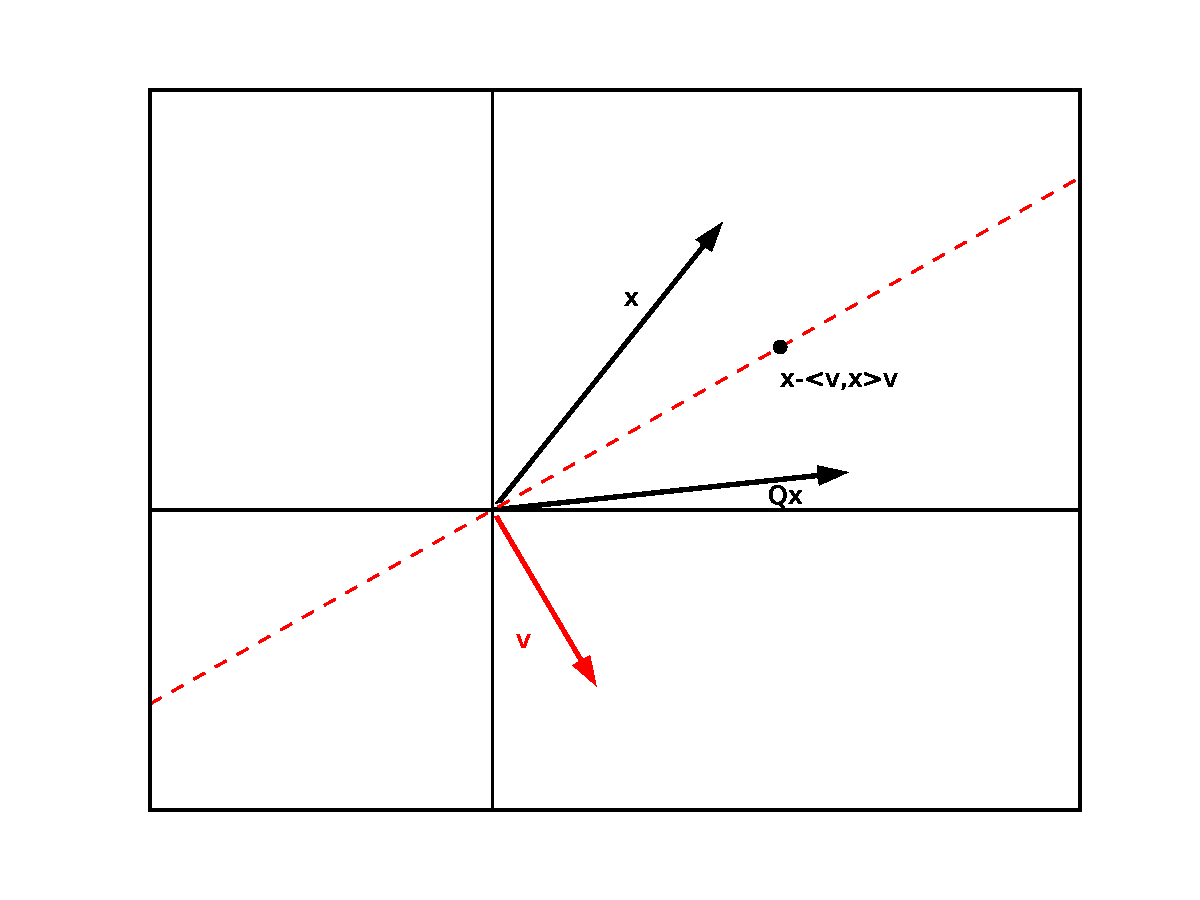
\includegraphics[width= \textwidth]{fig1}
\caption{Householder reflector}
\label{fig:Householder_reflector}
\end{figure}

\subsection*{Householder triangularization}
Consider the problem of computing the $QR$ decomposition of a matrix $A$.
You've already learned the Gram-Schmidt and the Modified Gram-Schmidt algorithms for this problem.
The $QR$ decomposition can also be computed by applying a series of Householder reflections.
Gram-Schmidt and Modified Gram-Schmidt make $A$ \emph{orthonormal} using a series of transformations stored in an \emph{upper triangular} matrix.
On the other hand, we can use Householder reflections to make $A$ \emph{triangular} by a series of \emph{orthonormal} transformations.

Let's demonstrate this method on a $4 \times 3$ matrix $A$.
First we find an orthonormal transformation $Q_1$ that maps the first column of A into the span of $e_1$
(where $e_1$ is the vector where the first element is one and the remainder of the elements are zeros).

\def\mc#1{\multicolumn{1}{c|}{#1}}
\begin{equation*}
\begin{pmatrix}
* & * & * \\
* & * & * \\
* & * & * \\
* & * & *
\end{pmatrix}
\underrightarrow{Q_1}
\begin{pmatrix}

* & * & * & \\ \cline{2-3}
\mc{0} & * & \mc{*}& \\
\mc{0} & * & \mc{*} & \\
\mc{0}& * & \mc{*} & \\ \cline{2-3}
\end{pmatrix}
\end{equation*}
Let $A_2$ be the boxed submatrix of $A$.
Now find an orthonormal transformation $Q_2$ that maps the first column of $A_2$ into the span of $e_2$.

\begin{equation*}
\begin{pmatrix}
* & * \\
* & * \\
* & *
\end{pmatrix}
\underrightarrow{Q_2}
\begin{pmatrix}
* & * \\
0 & * \\
0 & *
\end{pmatrix}
\end{equation*}
Similarly, $ \begin{pmatrix} * \\ * \end{pmatrix} \underrightarrow{Q_3} \begin{pmatrix} * \\ 0 \end{pmatrix} $.
(Technically $Q_2$ and $Q_3$ act on the whole matrix and not just on the submatrices, so that $Q_i: \mathbb{R}^n \rightarrow \mathbb{R}^n$ for all $i$.
$Q_2$ leaves the first row and the first column alone, and $Q_3$ leaves the first two rows and the first two columns alone.)
Then $Q_3 Q_2 Q_1 A =$

\begin{equation*}
Q_3 Q_2 Q_1
\begin{pmatrix}
* & * & * \\
* & * & * \\
* & * & * \\
* & * & *
\end{pmatrix}
= Q_3 Q_2
\begin{pmatrix}
* & * & * \\
0 & * & * \\
0 & * & * \\
0 & * & *
\end{pmatrix}
= Q_3
\begin{pmatrix}
* & * & * \\
0 & * & * \\
0 & 0 & * \\
0 & 0 & *
\end{pmatrix}
=
\begin{pmatrix}
* & * & * \\
0 & * & * \\
0 & 0 & * \\
0 & 0 & 0
\end{pmatrix}
\end{equation*}

We've accomplished our goal, which was to triangularize $A$ using orthonormal transformations.
But how do we find the $Q_i$ that do what we want? The answer lies in using Householder reflections.

To find $Q_1$, we first identify an appropriate hyperplane to reflect $x$ into the span of $e_1$.
It turns out there are two hyperplanes that will work, as shown in figure \ref{fig:two reflectors}.
(In the complex case, there are infinitely many such hyperplanes.)
Between the two, the one that reflects $x$ further will be more numerically stable.
This is the hyperplane perpendicular to $v = sign(x_1)\norm{x}_2 e_1 + x$.

To see how this works, let $x$ be the first column of the submatrix that we want to project onto the span of $e_1$.
In order for this to be a unitary operation, this will need to preserve the norm of $x$.
This means that $\left( I - 2 v v^\mathsf{H} \right) x = \pm \norm{x} e_1$, or, in other words,

\[ 2 v v^\mathsf{H} x =
\begin{pmatrix}
x_1 \pm \norm{x} \\
x_2 \\
x_3 \\
\vdots \\
x_n
\end{pmatrix}\]

Let $u$ be the vector on the right hand side of this expression.
It can be shown that the vector  $\frac{u}{\norm{u}}$ is the proper choice for $v$.
%We will show that the vector $\frac{u}{\norm{u}}$ is the proper choice for $v$.
%Notice that:
%
%\[\norm{u}^2 = \norm{x}^2 \pm 2 \norm{x} x_1 + x_1^2 + x_2 + \dots + x_n^2 = 2 \norm{x}^2 \pm 2 \norm{x} x_1 \]
%
%and that
%
%\[\norm{x}^2 \pm \norm{x} x_1 = u^\mathsf{H} x \]
%
%So we have
%
%\begin{align*}
%2 v v^\mathsf{H} x &= 2 u \frac{\norm{x}^2 \pm x_1 \norm{x}}{\norm{u}^2} \\
%		&= 2 u \frac{u^\mathsf{H} x}{\norm{u}^2} \\
%		&= 2 \frac{u}{\norm{u}} \left( \frac{u}{\norm{u}} \right)^\mathsf{H} x
%\end{align*}
%
%So $\frac{u}{\norm{u}}$ is a proper choice of $v$ that will project $x$ into the span of $e_1$.

This whole process is summarized in Algorithm \ref{Alg:Householder}.

\begin{figure}
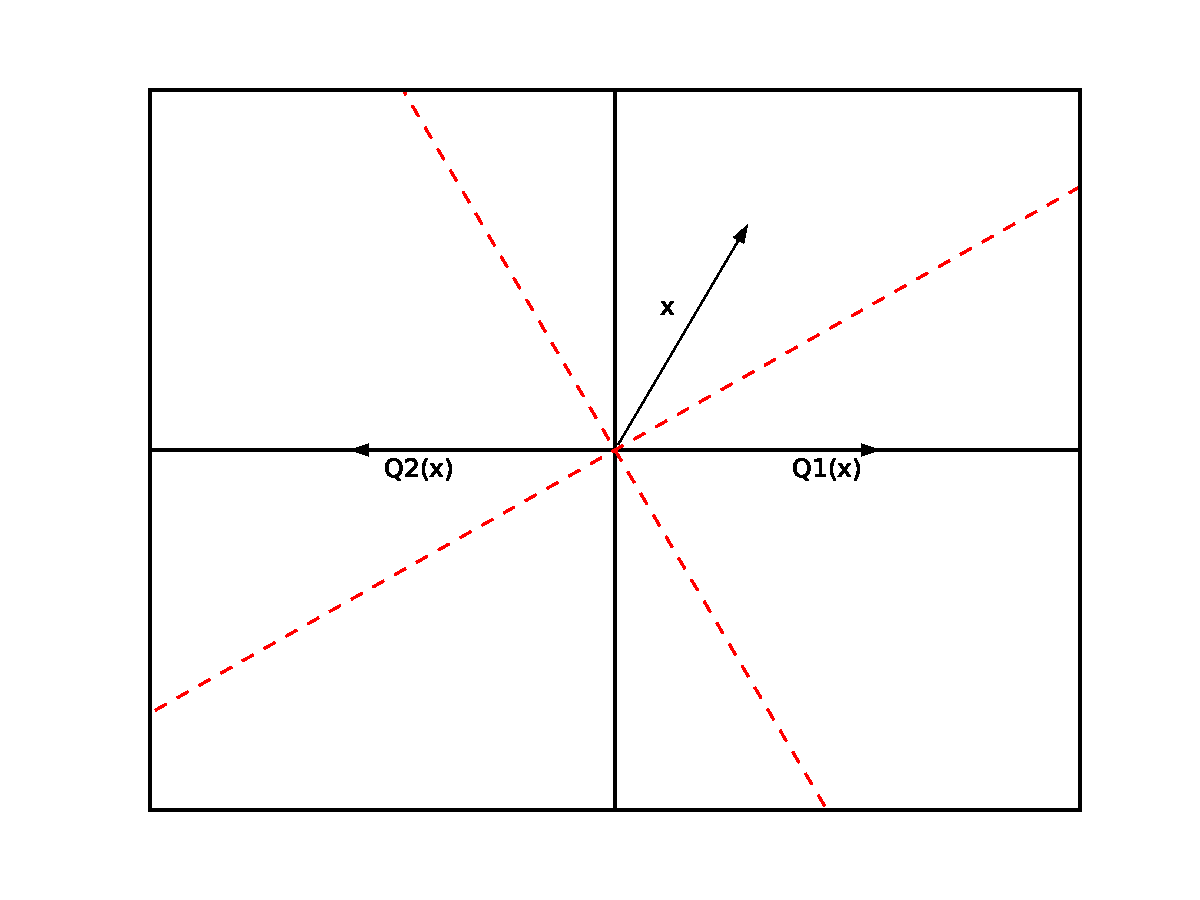
\includegraphics[width= \textwidth]{fig2}
\caption{two reflectors}
\label{fig:two reflectors}
\end{figure}

\begin{algorithm}
\caption{Householder triangularization}
\label{Alg:Householder}
\begin{algorithmic}[1]
\Procedure{Householder}{$A$}
\State $m, n \gets \text{shape} \left( A \right)$
\State $R \gets \text{copy} \left( A \right)$
\State $Q \gets I_m$
\For{$0 \leq k < n-1$}
    \State $v_k \gets \text{copy} \left( R_{k:,k} \right)$
    \State $v_{k_0} \gets v_{k_0} + \text{sign} \left( v_{k_0} \right) \norm{v_k}$
    \State $v_k \gets v_k / \norm{v_k}$
    \State $R_{k:,k:} \gets R_{k:,k:} - 2 v_k \left( v_k^\mathsf{H} R_{k:,k:} \right)$
    \State $Q_{k:} \gets Q_{k:} - 2 v_k \left( v_k^\mathsf{H} Q_{k:} \right)$
\EndFor
\State \pseudoli{return} $Q^\mathsf{H}, R$
\EndProcedure
\end{algorithmic}
\end{algorithm}

To see how we are operating on the matrices $A$ and $Q$, consider the way each orthonormal transformation defined by the $v_k$ operates blockwise on each matrix.
The matrix form of each operation on $A$ and $Q$ can be represented in block form like this:

\[
\begin{pmatrix}
I & 0 \\
0 & I - 2 v_k v_k^\mathsf{H}
\end{pmatrix}
\]

Notice that a block matrix of this form operates only on entries that lie in the rows from $k$ onward.
Consider what happens when we left-multiply a $m \times n$ matrix by a block matrix of this form.
We obtain the following:

\[
\begin{pmatrix}
I & 0 \\
0 & I - 2 v_k v_k^\mathsf{H}
\end{pmatrix}
\cdot
\begin{pmatrix}
A[:k,:k] & A[:k,k:] \\
A[k:,:k] & A[k:,k:]
\end{pmatrix}
=
\begin{pmatrix}
A[:k,:k] & A[:k,k:] \\
A[k:,:k] - 2 v_k v_k^\mathsf{H} A[k:,:k] & A[k:,k:] - 2 v_k v_k^\mathsf{H} A[k:,k:]
\end{pmatrix}
\]

And, when we consider right multiplication by the same block matrix, we see that it fixes the first $k-1$ columns as below.

\[
\begin{pmatrix}
A[:k,:k] & A[:k,k:] \\
A[k:,:k] & A[k:,k:]
\end{pmatrix}
\cdot
\begin{pmatrix}
I & 0 \\
0 & I - 2 v_k v_k^\mathsf{H}
\end{pmatrix}
=
\begin{pmatrix}
A[:k,:k] & A[:k,k:] - 2  A[:k,k:] v_k v_k^\mathsf{H} \\
A[k:,:k] & A[k:,k:] - 2 A[k:,k:] v_k v_k^\mathsf{H}
\end{pmatrix}
\]

When we are iterating through the columns of $R$ and zeroing out the entries below the main diagonal we are able to safely ignore all the entries that lie in columns we have already processed because they are already zero.

This algorithm returns orthonormal $Q$ and upper triangular $R$ satisfying $A = QR$.
Notice that we did not explicitly construct each orthonormal reflector matrix.
We applied the changes we needed to each portion of the array that needed to be changed.
Doing the operations in this way allows us to avoid unnecessarily increasing the computational complexity of the algorithm.
A few other clever optimizations can still be applied, but they will not change the overall complexity of the algorithm.

%It should now be clear how it was that we computed $R$ using this algorithm.
%$Q$ is computed in much the same way.
%Since each of the orthonormal operations is self-inverse (i.e. idempotent), $Q$ can be computed by applying the these operations to the identity in reverse order.
%In other words, you could make an identity matrix and then for $k$ such that $n-2 \geq k > -1$ , do $I[k:,k:] -= 2 v_k v_k^\mathsf{H}$
%In our computation, it may be more convenient to simply apply the operations to an identity matrix as we go, just like we are doing to $R$, then take the transpose at the end to invert $Q$.
%This way we do not have to store the $v_k$ as we go.
%There is one key difference, when applying these operations to $Q$ we cannot ignore columns we have already processed because they are not necessarily zero.
%It is interesting to note that we can use the $v_k$ to behave like $Q$ or $Q^{-1}$ depending on the order in which we apply them.
%Such an approach does not require the computation of $Q$ or $Q^{-1}$ at all.

Another important thing to notice is that an outer product is needed to compute
$v_k \left( v_k^\mathsf{H} A[k:,k:] \right)$, not an inner product.
Make sure that you account for this when you write the code to run this algorithm.
You can either make the vectors $v_k$ column vectors (two dimensional with a single column) instead of just one-dimensional arrays, or you can use the built in function \li{np.outer} in the appropriate place.

\begin{problem}
\label{prob:HouseholderQR}
Write a function \li{householder} that accepts an array $A$ as input, and performs
the algorithm described above to compute the QR decomposition of $A$. Return the
matrices $Q$ and $R$.

It is simple to check that your code works: multiply the two output matrices
of your function, and check that the result matches the original input matrix.
\end{problem}

\subsection*{Stability of the Householder QR algorithm}
We will now examine the stability of the Householder QR algorithm.
We will use SciPy's built in QR factorization which uses Householder reflections internally.

Try the following in Python.

\begin{lstlisting}
>>> import numpy as np
>>> from numpy.random import rand
>>> from scipy import linalg as la
>>> Q, X = la.qr(rand(500,500)) # create a random orthonormal matrix:
>>> R = np.triu(rand(500,500)) # create a random upper triangular matrix
>>> A = np.dot(Q,R) # Q and R are the exact QR decomposition of A
>>> Q1, R1 = la.qr(A) # compute QR decomposition of A
>>> la.norm(Q1-Q)/la.norm(Q) # check error in Q
0.282842955725
>>> la.norm(R1-R)/la.norm(R) # check error in R
0.0428922016647
\end{lstlisting}
This is terrible!
This algorithm works in $16$ decimal points of precision, but $Q_1$ and $R_1$ are only accurate to $0$ and $1$ decimal points, respectively.
We've lost $16$ decimal points of precision!

Don't lose hope.
Check how close the product $Q_1 R_1$ is to $A$.
\begin{lstlisting}
>>> A1 = Q1.dot(R1)
>>> np.absolute(A1 - A).max()
3.9968028886505635e-15
\end{lstlisting}
We've now recovered $15$ digits of accuracy.
Considering the error relative to the norm of $A$ (using the 2-norm for matrices), we see that this relative error is even smaller.
\begin{lstlisting}
>>> la.norm(A1 - A, ord=2) / la.norm(A, ord=2)
8.8655568331889288e-16
\end{lstlisting}
The errors in $Q_1$ and $R_1$ were somehow ``correlated," so that they canceled out in the product.
The errors in $Q_1$ and $R_1$ are called \emph{forward errors}.
The error in $A_1$ is the \emph{backward error}.

In fact, the large errors in \li{Q1} and \li{R1} were not because the algorithm was bad, it was because $A$ was poorly conditioned.
The condition number for randomly generated upper triangular matrices generally very high, and this was the case here.
This has, in turn, made the condition number of $A$ extremely large as well.
Try the following to compute the condition numbers of $A$.
In this case the condition numbers of $A$ and $R$ are computed to be different, though, in theory, they should be exactly the same.
\begin{lstlisting}
>>> from numpy.linalg import cond
>>> cond(A)
4.1426075832870472e+18
>>> cond(R)
3.1767577244363792e+19
\end{lstlisting}

Householder QR factorization is more numerically stable than Gram-Schmidt or even Modified Gram-Schmidt (MGS).
However, MGS is still useful for some types of iterative methods, because it finds the orthonormal basis one vector at a time instead of all at once (for an example see Lab \ref{lab:EigSolve}).

\subsection*{Upper Hessenberg Form}
An upper Hessenberg matrix is a square matrix with zeros below the first subdiagonal.
Every  $n \times n$ matrix $A$ can be written $A = Q^THQ$ where $Q$ is orthonormal and $H$ is an upper Hessenberg matrix, called the Hessenberg form of $A$.

The Hessenberg decomposition can be computed using Householder reflections, in a process very similar to Householder triangularization.
Let's demonstrate this process on a $5 \times 5$ matrix $A$.
Note that $A=Q^THQ$ is equivalent to $QAQ^T = H$; thus our strategy is to multiply $A$ on the right and left by a series of orthonormal matrices until it is in Hessenberg form.
If we try the same $Q_1$ as in the first step of the Householder algorithm, then with $Q_1 A$ we introduce zeros in the first column of $A$.
However, since we now have to multiply $Q_1 A$ on the left by $Q_1^T$, all those zeros are destroyed, as demonstrated below.
In order to zero out the entire first column we chose $Q_1$ so that it does not fix the first row.
When we apply the same operation on the right, this ruins the column that we just zeroed out.
(Although this process may seem futile now, it actually does tend to decrease the size of the subdiagonal entries.
If we repeat it over and over again, the subdiagonal entries will often converge to zero.
That's the idea behind the $QR$ algorithm in Lab \ref{lab:EigSolve}.)
\[
\begin{array}{ccccc}
\begin{pmatrix}
* & * & * & * & * \\
* & * & * & * & * \\
* & * & * & * & * \\
* & * & * & * & * \\
* & * & * & * & *
\end{pmatrix}
&\underrightarrow{Q_1 \cdot }&
\begin{pmatrix}
* & * & * & * & * \\
0 & * & * & * & * \\
0 & * & * & * & * \\
0 & * & * & * & * \\
0 & * & * & * & *
\end{pmatrix}
&\underrightarrow{\cdot Q_1^T }&
\begin{pmatrix}
* & * & * & * & * \\
* & * & * & * & * \\
* & * & * & * & * \\
* & * & * & * & * \\
* & * & * & * & *
\end{pmatrix}
\\
A & & Q_1A & & Q_1 A Q_1^T
  \end{array}
\]
Instead, let's try starting with a different $Q_1$ that leaves the \emph{first} row alone and reflects the \emph{rest} of the rows into the span of $e_2$. This means that $Q_1^T$ leaves the first column alone.
\[
\begin{array}{ccccc}
\begin{pmatrix}
* & * & * & * & * \\
* & * & * & * & * \\
* & * & * & * & * \\
* & * & * & * & * \\
* & * & * & * & *
\end{pmatrix}
&\underrightarrow{Q_1 \cdot }&
\begin{pmatrix}
* & * & * & * & * \\
* & * & * & * & * \\
0 & * & * & * & * \\
0 & * & * & * & * \\
0 & * & * & * & *
\end{pmatrix}
&\underrightarrow{\cdot Q_1^T }&
\begin{pmatrix}
* & * & * & * & * \\
* & * & * & * & * \\
0 & * & * & * & * \\
0 & * & * & * & * \\
0 & * & * & * & *
\end{pmatrix}
\\
A & & Q_1A & & Q_1 A Q_1^T
  \end{array}
\]
We now iterate through the matrix until we obtain
\begin{equation*}
Q_3 Q_2 Q_1 A Q_1^T Q_2 ^T Q_3^T =
\begin{pmatrix}
* & * & * & * & * \\
* & * & * & * & * \\
0 & * & * & * & * \\
0 & 0 & * & * & * \\
0 & 0 & 0 & * & *
\end{pmatrix}
\end{equation*}

This is even more convenient when we are working with Hermitian matrices.
In that case, the matrices applied on the left zero out everything below the first subdiagonal and the matrices applied on the right zero out everything above the first superdiagonal, leaving us with a tridiagonal matrix.
There are remarkably efficient ways to solve systems involving tridiagonal matrices, so this is especially convenient.

The pseudocode for computation of the Hessenberg form of a matrix is shown in Algorithm \ref{Alg:Hessenberg}.
The exact inner workings of this algorithm are similar to the inner workings of Algorithm \ref{Alg:Householder}.

\begin{algorithm}
\caption{Reduction to Hessenberg Form}
\label{Alg:Hessenberg}
\begin{algorithmic}[1]
\Procedure{Hessenberg}{$G,u,l,p$}
\State $m, n \gets \text{shape}(A)$
\State $H \gets \text{copy}(A)$
\State $Q \gets I_m$
\For{$0 \leq k < n-2$}
    \State $v_k \gets H_{k+1:, k}$
    \State $v_{k_0} \gets v_{k_0} + \text{sign}(v_{k_0}) \norm{v_k}$
    \State $v_k \gets v_k/norm{v_k}$
    \State $H_{k+1:,k:} \gets H_{k+1:,k:} - 2v_k(v_k^\mathsf{H} H_{k+1:,k:})$
    \State $H_{:,k+1:} \gets H_{:,k+1:} - 2(H_{:,k+1:} v_k) v_k^\mathsf{H}$
    \State $Q_{k+1:} \gets Q_{k+1:} - 2v_k(v_k^\mathsf{H} Q_{k+1:})$
\EndFor
\State \pseudoli{return} $Q, R$
\EndProcedure
\end{algorithmic}
\end{algorithm}

\begin{problem}
\label{prob:hessenberg}
Write a function \li{hessenberg} that computes the Hessenberg form of a real-valued
input matrix $A$. The function should return $Q$ and $H$ satisfying $A = Q^THQ$,
where $Q$ is orthonormal and $H$ has zeros below the first subdiagonal.

The code for this algorithm will be fairly similar to the code for the QR factorization using Householder reflections.
This factorization technique will be used later on in Lab \ref{lab:EigSolve}.
Notice what happens when you compute the Hessenberg factorization of a Hermitian matrix.
\end{problem}

%Sources: http://www.cs.unc.edu/~krishnas/eigen/node5.html
% http://en.wikipedia.org/wiki/Givens_rotation
%http://en.wikipedia.org/wiki/QR_decomposition
%	Note the Operation count: Householder is 2/3 n^3, MGS is 2 n^3
%http://en.wikipedia.org/wiki/QR_algorithm
%Applied Numerical methods using MATLAB by Yang has some code written for this
%http://www.math.kent.edu/~reichel/courses/intr.num.comp.2/lecture21/evmeth.pdf
%	These are eigenvalue algorithms explained carefully
%http://en.wikipedia.org/wiki/Householder_transformation
%Numerical Linear Algebra, by Lloyd N. Trefethen and David Bau III, Chapters 10 and 16 
